\documentclass{article}
\usepackage[margin=0.5in]{geometry}
\usepackage[utf8]{inputenc}
\usepackage{textcomp}
\usepackage{polski}

\usepackage{pgfplots}
\pgfplotsset{width=18cm,compat=1.9}
%\usepgfplotslibrary{external}
%\tikzexternalize

\begin{document}

\section*{Porównanie wydajności drzew van Emde Boasa, x-fast oraz y-fast}
Mateusz Lewko \\

\textbf{Wykonane prace}
Zaimplementowałem trzy struktury danych z wykładu:

\begin{itemize}
  \item drzewo van Emde Boasa (\texttt{v-eb.h}), 
  \item x-fast trie (\texttt{x-fast.h}),
  \item y-fast trie wykorzystujące x-fast oraz drzewo bst (\texttt{y-fast.h}),
\end{itemize}
oraz wrapper na std::set (dla porównania, jest w pliku (\texttt{test.h})).

Każda ze struktur implementuje taki sam interfejs (lookup, successor,
insert --- plik (\texttt{interface.h})).
Konstruktor każdej struktury przyjmuje wykładnik $k$ z rozmiaru uniwersum $U = 2^k$.
Jeśli w strukturze nie ma następnika dla danego zapytania, to zwracane jest $U$.
Zarządzanie pamięcią jest zapewnione przez użycie shared pointerów. Skutkiem ubocznym
użycia shared pointerów jest duża stała wykonywanych operacji.

Poprawność zaimplementowanych metod jest sprawdzana poprzez wypisanie xora
wyników operacji \textit{successor} dla każdej struktury.

\textbf{Testowanie}
Dla danego $N$ losowane jest $N$ liczb jako wejście do operacji insert oraz
lookup, a następnie $N$ liczb na
których kolejno wykonywane są zapytania o następnika. Liczby są
jednostajnie losowane z przedziału $[0, U)$. We wszystkich testach przyjęto
$U = 2^{25}$. Mierzony jest sumaryczny czas wykonania wszystkich operacji
(z podziałem na typ operacji).

\textbf{Kompilacja} Wszystkie testy można skompilować jednym poleceniem w
systemie linux: \texttt{g++ test.cpp -o test -O3 -Wall -Wextra -std=c++17},
a następnie uruchomić: \texttt{./test}.

\textbf{Wnioski} Dostępy do pamięci i inne kosztowne operacje nie dają tak
dużej różnicy w czasie działania jak można byłoby oczekiwać od złożoności $O(\log \log U)$.
Drzewo van Emde Boasa okazało się najszybsze dla każdych danych testowych, jednak
bardzo duże zużycie pamięci oznacza małą przydatność w praktyce oraz długi czas
tworzenia struktury (alokowanie pamięci). 
Implementacja drzewa y-fast okazała się mieć na tyle dużą
stałą, że jej sumaryczny czas działania jest większy niż struktury std::set z biblioteki
standardowej C++ (o gorszej złożoności operacji successor). 
Drzewa x-fast wypadły najlepiej pod względem czasu wykonania i wyprzedzają std::set już
dla danych rzędu $2 * 10^6$.

Na końcu pliku \texttt{test.cpp} znajduje się zakomentowany wynik programu.
Czasy działania poszczególnych operacji zostały przedstawione na poniższych 
wykresach. 

\begin{figure}
  \centering
  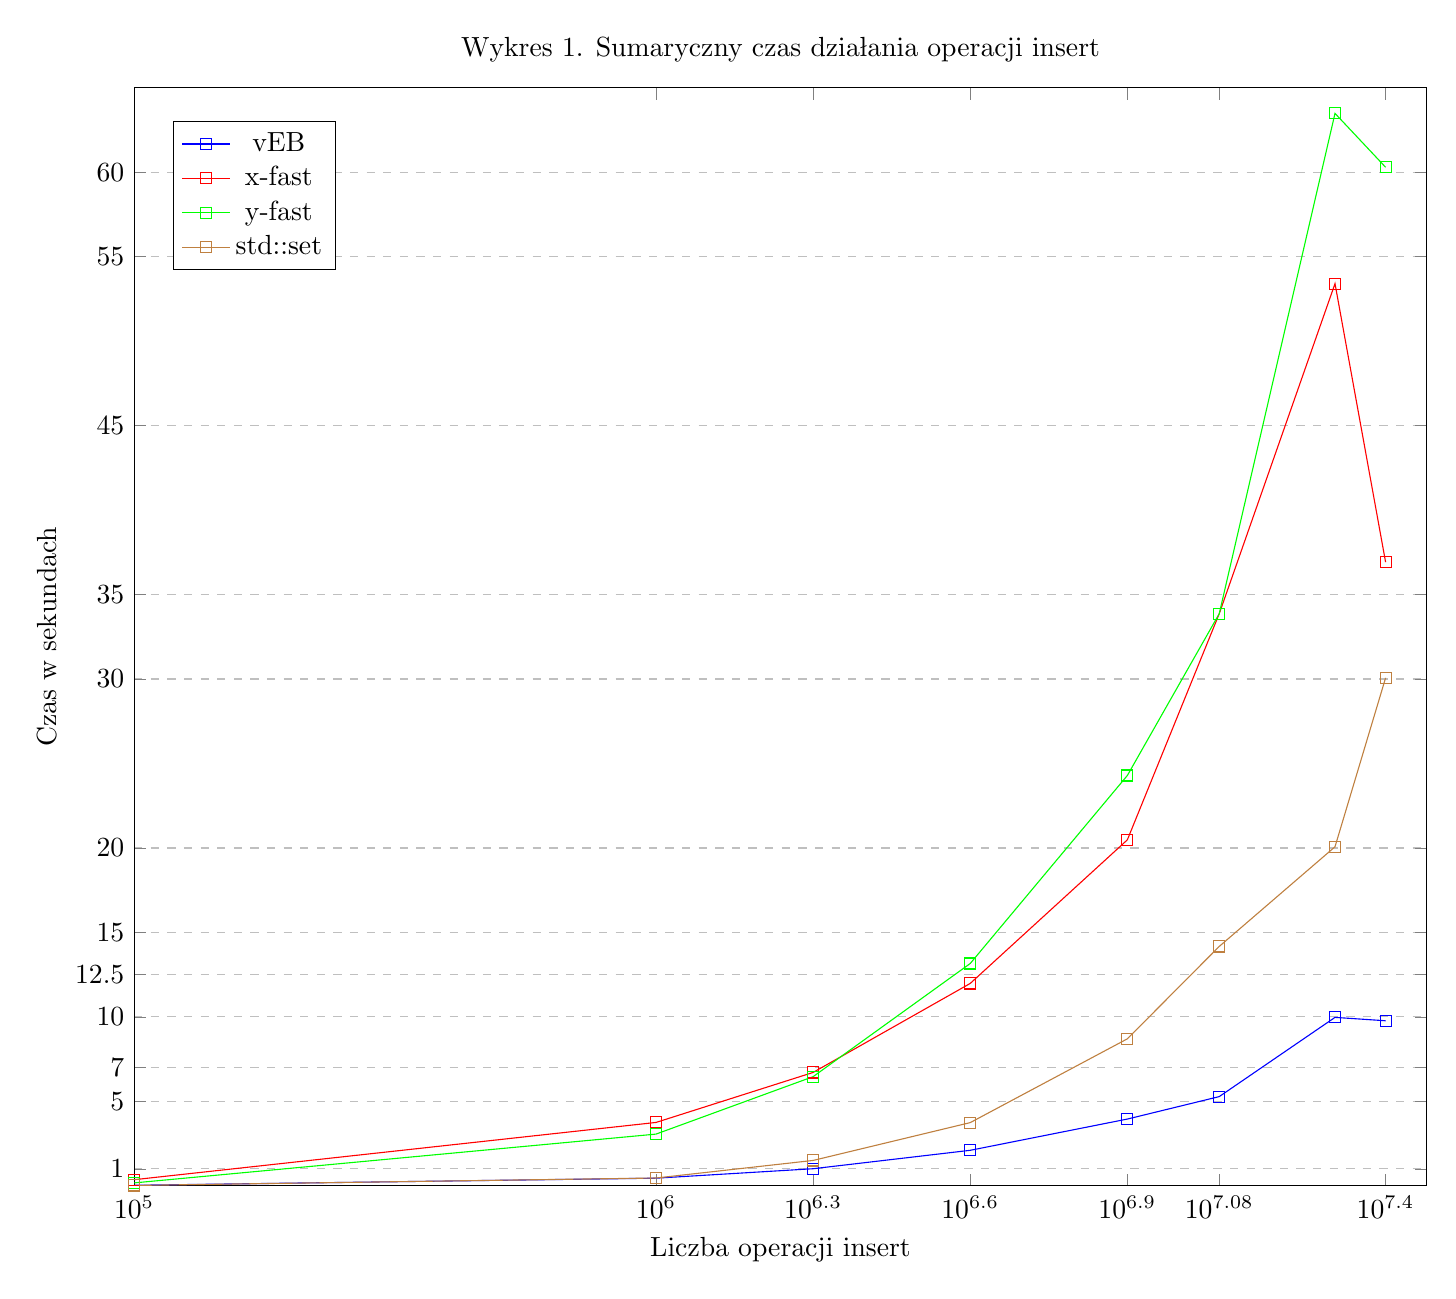
\begin{tikzpicture}
    \begin{semilogxaxis}[
        title={Wykres 1. Sumaryczny czas działania operacji insert},
        xlabel={Liczba operacji insert},
        ylabel={Czas w sekundach},
        xmin=100000, xmax=30000000,
        ymin=0, ymax=65,
        xtick={100000, 1000000, 2000000, 4000000, 8000000, 12000000, 25000000},
        ytick={1, 5, 7, 10, 12.5, 15, 20, 30, 35, 45, 55, 60 },
        legend pos=north west,
        ymajorgrids=true,
        grid style=dashed,
      ]

      \addplot[
        color=blue,
        mark=square,
      ]
      coordinates {
          (100000, 0.03)(1000000, 0.45)(2000000, 1.01)(4000000, 2.1)
          (8000000, 3.95)(12000000, 5.28)(20000000, 9.97)(25000000, 9.77)
        };

      \addplot[
        color=red,
        mark=square,
      ]
      coordinates {
          (100000, 0.36)(1000000, 3.75)(2000000, 6.71)(4000000, 11.98)
          (8000000, 20.48)(12000000, 33.87)(20000000, 53.41)(25000000, 36.92)
        };

      \addplot[
        color=green,
        mark=square,
      ]
      coordinates {
          (100000, 0.17)(1000000, 3.06)(2000000, 6.46)(4000000, 13.16)
          (8000000, 24.29)(12000000, 33.87)(20000000, 63.49)(25000000, 60.3)
        };

      \addplot[
        color=brown,
        mark=square,
      ]
      coordinates {
          (100000, 0.02)(1000000, 0.46)(2000000, 1.5)(4000000, 3.74)
          (8000000, 8.7)(12000000, 14.17)(20000000, 20.07)(25000000, 30.07)
        };

      \legend{vEB, x-fast, y-fast, std::set}

    \end{semilogxaxis}
  \end{tikzpicture}
\end{figure}

\begin{figure}
  \centering
  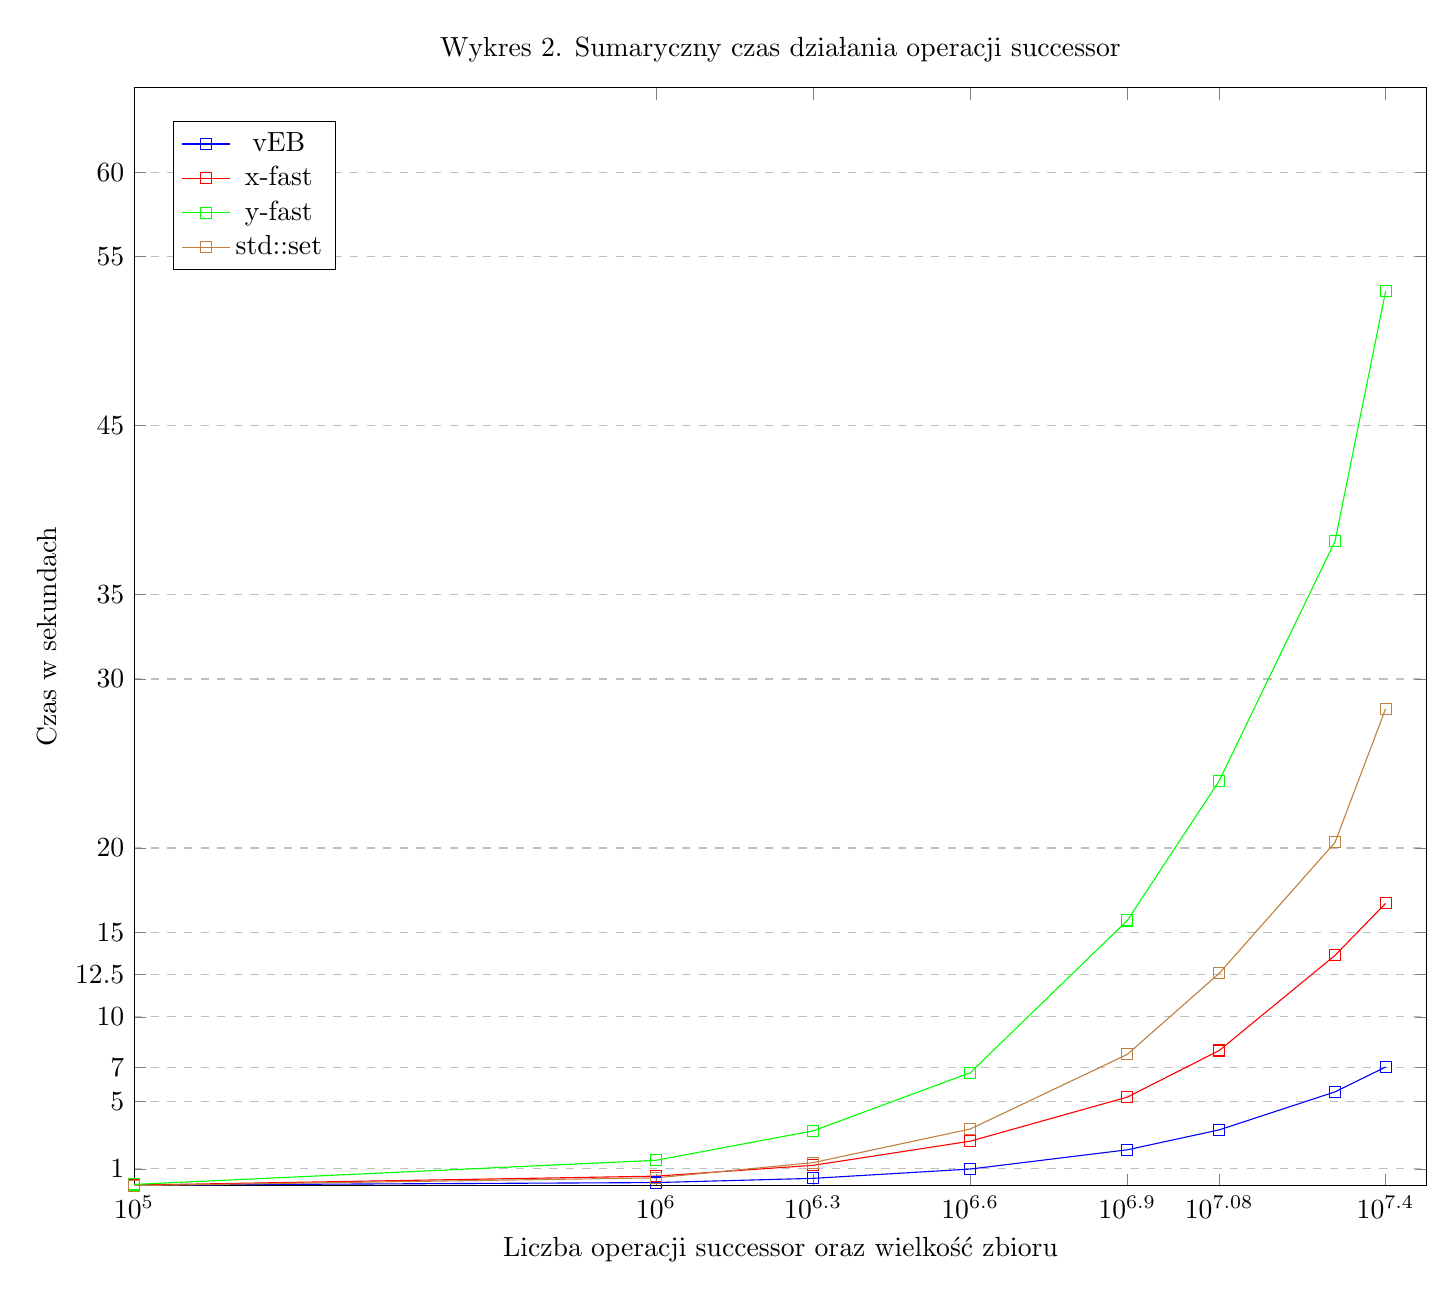
\begin{tikzpicture}
    \begin{semilogxaxis}[
        title={Wykres 2. Sumaryczny czas działania operacji successor},
        xlabel={Liczba operacji successor oraz wielkość zbioru},
        ylabel={Czas w sekundach},
        xmin=100000, xmax=30000000,
        ymin=0, ymax=65,
        xtick={100000, 1000000, 2000000, 4000000, 8000000, 12000000, 25000000},
        ytick={1, 5, 7, 10, 12.5, 15, 20, 30, 35, 45, 55, 60 },
        legend pos=north west,
        ymajorgrids=true,
        grid style=dashed,
      ]

      \addplot[
        color=blue,
        mark=square,
      ]
      coordinates {
          (100000, 0.04)(1000000, 0.19)(2000000, 0.44)(4000000, 0.99)
          (8000000, 2.13)(12000000, 3.31)(20000000, 5.56)(25000000, 7.03)
        };

      \addplot[
        color=red,
        mark=square,
      ]
      coordinates {
          (100000, 0.04)(1000000, 0.57)(2000000, 1.21)(4000000, 2.64)
          (8000000, 5.25)(12000000, 8.01)(20000000, 13.64)(25000000, 16.72)
        };

      \addplot[
        color=green,
        mark=square,
      ]
      coordinates {
          (100000, 0.08)(1000000, 1.51)(2000000, 3.25)(4000000, 6.69)
          (8000000, 15.71)(12000000, 23.98)(20000000, 38.16)(25000000, 52.95)
        };

      \addplot[
        color=brown,
        mark=square,
      ]
      coordinates {
          (100000, 0.01)(1000000, 0.47)(2000000, 1.37)(4000000, 3.36)
          (8000000, 7.78)(12000000, 12.58)(20000000, 20.33)(25000000, 28.24)
        };

      \legend{vEB, x-fast, y-fast, std::set}

    \end{semilogxaxis}
  \end{tikzpicture}
\end{figure}


\begin{figure}
  \centering
  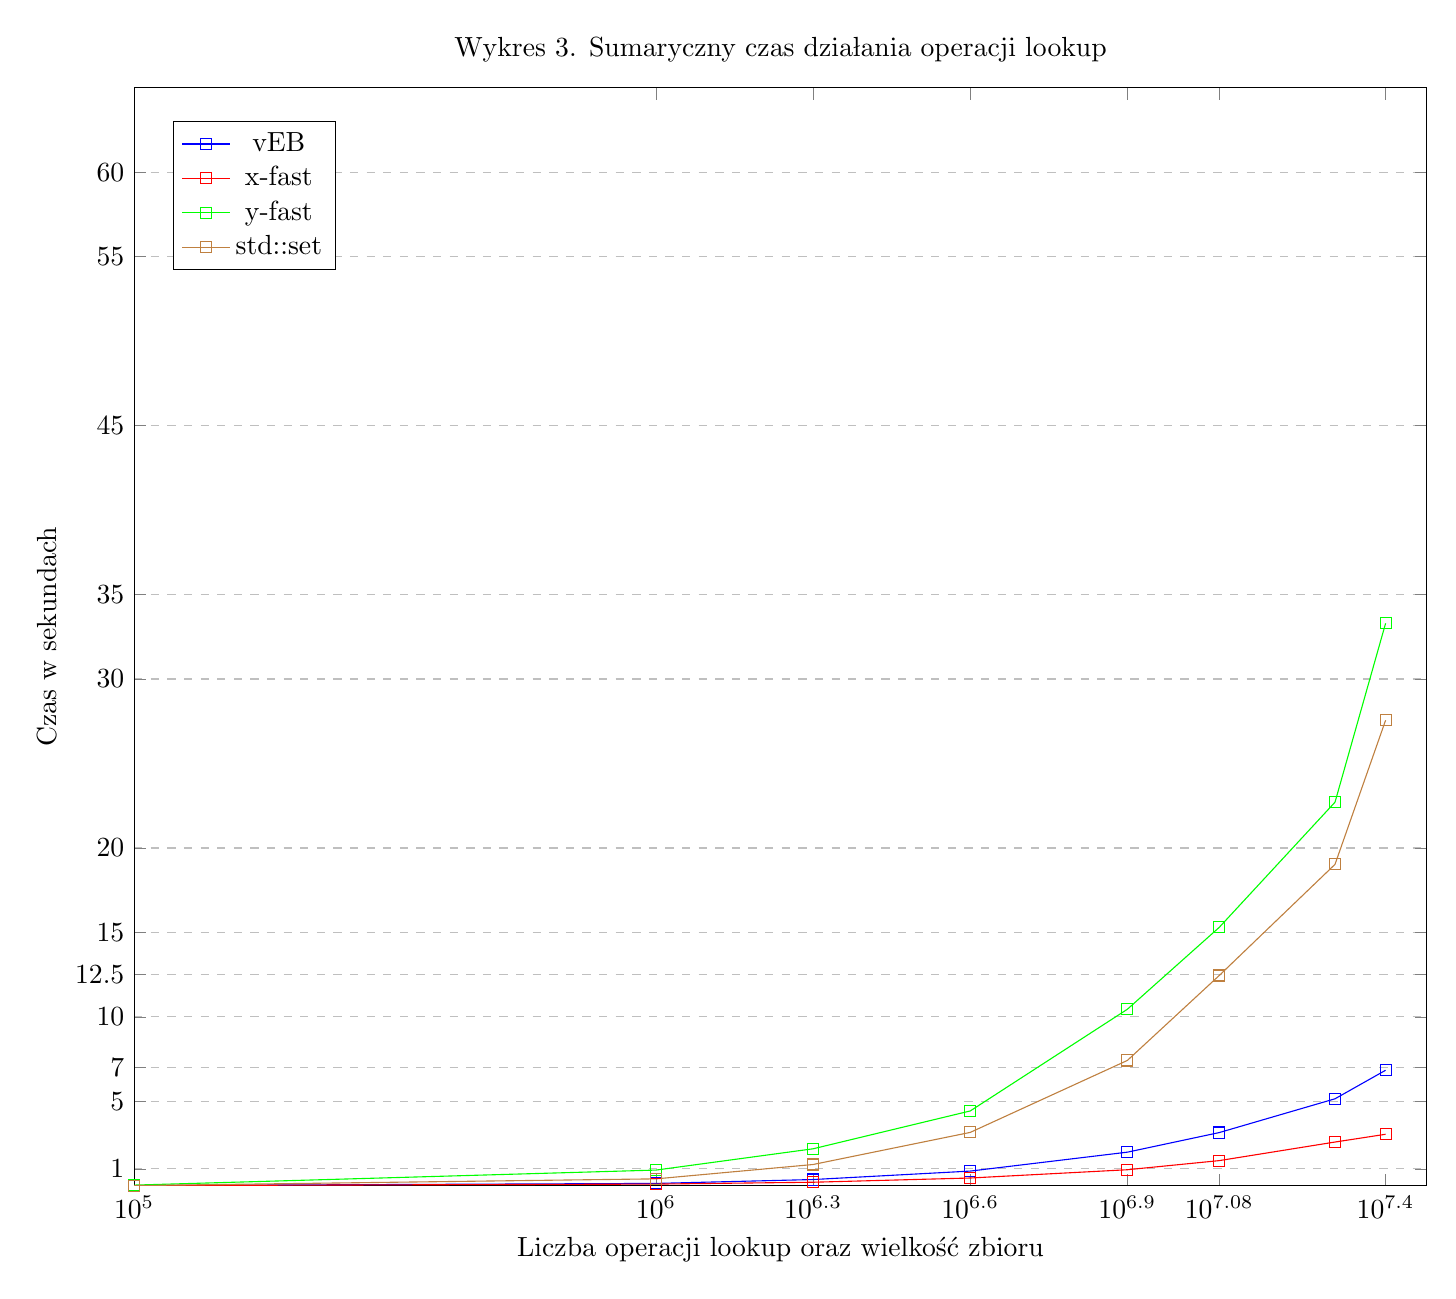
\begin{tikzpicture}
    \begin{semilogxaxis}[
        title={Wykres 3. Sumaryczny czas działania operacji lookup},
        xlabel={Liczba operacji lookup oraz wielkość zbioru},
        ylabel={Czas w sekundach},
        xmin=100000, xmax=30000000,
        ymin=0, ymax=65,
        xtick={100000, 1000000, 2000000, 4000000, 8000000, 12000000, 25000000},
        ytick={1, 5, 7, 10, 12.5, 15, 20, 30, 35, 45, 55, 60 },
        legend pos=north west,
        ymajorgrids=true,
        grid style=dashed,
      ]

      \addplot[
        color=blue,
        mark=square,
      ]
      coordinates {
          (100000, 0.01)(1000000, 0.14)(2000000, 0.37)(4000000, 0.87)
          (8000000, 1.99)(12000000, 3.15)(20000000, 5.15)(25000000, 6.84)
        };

      \addplot[
        color=red,
        mark=square,
      ]
      coordinates {
          (100000, 0.01)(1000000, 0.10)(2000000, 0.21)(4000000, 0.46)
          (8000000, 0.95)(12000000, 1.49)(20000000, 2.59)(25000000, 3.05)
        };

      \addplot[
        color=green,
        mark=square,
      ]
      coordinates {
          (100000, 0.04)(1000000, 0.93)(2000000, 2.19)(4000000, 4.43)
          (8000000, 10.45)(12000000, 15.30)(20000000, 22.71)(25000000, 33.30)
        };

      \addplot[
        color=brown,
        mark=square,
      ]
      coordinates {
          (100000, 0.01)(1000000, 0.41)(2000000, 1.26)(4000000, 3.16)
          (8000000, 7.42)(12000000, 12.45)(20000000, 19.03)(25000000, 27.56)
        };

      \legend{vEB, x-fast, y-fast, std::set}

    \end{semilogxaxis}
  \end{tikzpicture}
\end{figure}

\end{document}
